Hawick está 15 kilómetros al sur de Abbotsford,
y Kelso está 17 kilómetros al este de Abbotsford,
como se muestran a continuación en la figura \ref{fig:proverb_pitagoras_08}
\begin{figure}[H]
    \begin{center}
        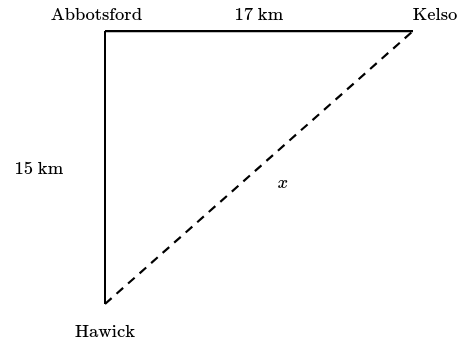
\includegraphics[width=0.5\textwidth]{../images/proverb_pitagoras_08.png}
    \end{center}
    \caption{}
    \label{fig:proverb_pitagoras_08}
\end{figure}
\textbf{¿Cuál es la distancia entre Hawick y Kelso?}\\
\textit{Redondea tu respuesta a la décima de kilómetro más cercana.}

\begin{solutionbox}{10cm}
    Podemos usar el teorema de Pitágoras para obtener $x$.
    La ecuación del teorema de Pitágoras es:
    \[c^2=a^2+b^2\]
    donde $a$ y $b$ son las longitudes de los dos catetos del triángulo y $c$ es la longitud de la hipotenusa.
    En este caso, $a=15$, $b=17$ y $c=x$.
    \begin{align*}
        x^2 & =15^2+17^2  \\
        x^2 & =514        \\
        x   & =\sqrt{514} \\
        x   & \sim 22.7
    \end{align*}
    La distancia de Hawick a Kelso es aproximadamente 22.7 kilómetros.
\end{solutionbox}